\documentclass[12pt]{article}
\usepackage[left=1cm, right=1cm, top=2cm,bottom=1.5cm]{geometry} 

\usepackage[parfill]{parskip}
\usepackage[utf8]{inputenc}
\usepackage[T2A]{fontenc}
\usepackage[russian]{babel}
\usepackage{enumitem}
\usepackage[normalem]{ulem}
\usepackage{amsfonts, amsmath, amsthm, amssymb, mathtools,xcolor}
\usepackage{blkarray}

\usepackage{tabularx}
\usepackage{hhline}

\usepackage{accents}
\usepackage{fancyhdr}
\pagestyle{fancy}
\renewcommand{\headrulewidth}{1.5pt}
\renewcommand{\footrulewidth}{1pt}

\usepackage{graphicx}
\usepackage[figurename=Рис.]{caption}
\usepackage{subcaption}
\usepackage{float}

%%Наименование папки откуда забирать изображения
\graphicspath{ {./images/} }

%%Изменение формата для ввода доказательства
\renewcommand{\proofname}{$\square$  \nopunct}
\renewcommand\qedsymbol{$\blacksquare$}

%%Изменение отступа на таблицах
\addto\captionsrussian{%
	\renewcommand{\proofname}{$\square$ \nopunct}%
}
%% Римские цифры
\newcommand{\RN}[1]{%
	\textup{\uppercase\expandafter{\romannumeral#1}}%
}

%% Для удобства записи
\newcommand{\MR}{\mathbb{R}}
\newcommand{\MC}{\mathbb{C}}
\newcommand{\MQ}{\mathbb{Q}}
\newcommand{\MN}{\mathbb{N}}
\newcommand{\MZ}{\mathbb{Z}}
\newcommand{\MTB}{\mathbb{T}}
\newcommand{\MTI}{\mathbb{I}}
\newcommand{\MI}{\mathrm{I}}
\newcommand{\MCI}{\mathcal{I}}
\newcommand{\MJ}{\mathrm{J}}
\newcommand{\MH}{\mathrm{H}}
\newcommand{\MT}{\mathrm{T}}
\newcommand{\MU}{\mathcal{U}}
\newcommand{\MV}{\mathcal{V}}
\newcommand{\MB}{\mathcal{B}}
\newcommand{\MF}{\mathcal{F}}
\newcommand{\MW}{\mathcal{W}}
\newcommand{\ML}{\mathcal{L}}
\newcommand{\MP}{\mathcal{P}}
\newcommand{\VN}{\varnothing}
\newcommand{\VE}{\varepsilon}
\newcommand{\dx}{\, dx}
\newcommand{\dy}{\, dy}
\newcommand{\dz}{\, dz}
\newcommand{\dd}{\, d}


\theoremstyle{definition}
\newtheorem{defn}{Опр:}
\newtheorem{rem}{Rm:}
\newtheorem{prop}{Утв.}
\newtheorem{exrc}{Упр.}
\newtheorem{problem}{Задача}
\newtheorem{lemma}{Лемма}
\newtheorem{theorem}{Теорема}
\newtheorem{corollary}{Следствие}

\newenvironment{cusdefn}[1]
{\renewcommand\thedefn{#1}\defn}
{\enddefn}

\DeclareRobustCommand{\divby}{%
	\mathrel{\text{\vbox{\baselineskip.65ex\lineskiplimit0pt\hbox{.}\hbox{.}\hbox{.}}}}%
}
\DeclareRobustCommand{\ndivby}{\mkern-1mu\not\mathrel{\mkern4.5mu\divby}\mkern1mu}


%Короткий минус
\DeclareMathSymbol{\SMN}{\mathbin}{AMSa}{"39}
%Длинная шапка
\newcommand{\overbar}[1]{\mkern 1.5mu\overline{\mkern-1.5mu#1\mkern-1.5mu}\mkern 1.5mu}
%Функция знака
\DeclareMathOperator{\sgn}{sgn}

%Функция ранга
\DeclareMathOperator{\rk}{\text{rk}}
\DeclareMathOperator{\diam}{\text{diam}}


%Обозначение константы
\DeclareMathOperator{\const}{\text{const}}

\DeclareMathOperator{\codim}{\text{codim}}

\DeclareMathOperator*{\dsum}{\displaystyle\sum}
\newcommand{\ddsum}[2]{\displaystyle\sum\limits_{#1}^{#2}}

%Интеграл в большом формате
\DeclareMathOperator{\dint}{\displaystyle\int}
\newcommand{\ddint}[2]{\displaystyle\int\limits_{#1}^{#2}}
\newcommand{\ssum}[1]{\displaystyle \sum\limits_{n=1}^{\infty}{#1}_n}

\newcommand{\smallerrel}[1]{\mathrel{\mathpalette\smallerrelaux{#1}}}
\newcommand{\smallerrelaux}[2]{\raisebox{.1ex}{\scalebox{.75}{$#1#2$}}}

\newcommand{\smallin}{\smallerrel{\in}}
\newcommand{\smallnotin}{\smallerrel{\notin}}

\newcommand*{\medcap}{\mathbin{\scalebox{1.25}{\ensuremath{\cap}}}}%
\newcommand*{\medcup}{\mathbin{\scalebox{1.25}{\ensuremath{\cup}}}}%

\makeatletter
\newcommand{\vast}{\bBigg@{3.5}}
\newcommand{\Vast}{\bBigg@{5}}
\makeatother

%Промежуточное значение для sup\inf, поскольку они имеют разную высоту
\newcommand{\newsup}{\mathop{\smash{\mathrm{sup}}}}
\newcommand{\newinf}{\mathop{\mathrm{inf}\vphantom{\mathrm{sup}}}}

%Скалярное произведение
\newcommand{\inner}[2]{\left\langle #1, #2 \right\rangle }
\newcommand{\linsp}[1]{\left\langle #1 \right\rangle }
\newcommand{\linmer}[2]{\left\langle #1 \vert #2\right\rangle }

%Подпись символов снизу
\newcommand{\ubar}[1]{\underaccent{\bar}{#1}}

%% Шапка для букв сверху
\newcommand{\wte}[1]{\widetilde{#1}}
\newcommand{\wht}[1]{\widehat{#1}}
\newcommand{\ovl}[1]{\overline{#1}}

%%Трансформация Фурье
\newcommand{\fourt}[1]{\mathcal{F}\left(#1\right)}
\newcommand{\ifourt}[1]{\mathcal{F}^{-1}\left(#1\right)}

%%Символ вектора
\newcommand{\vecm}[1]{\overrightarrow{#1\,}}

%%Пространстов матриц
\newcommand{\matsq}[1]{\operatorname{Mat}_{#1}}
\newcommand{\mat}[2]{\operatorname{Mat}_{#1, #2}}

%Оператор для действ и мнимых чисел
\DeclareMathOperator{\IM}{\operatorname{Im}}
\DeclareMathOperator{\RE}{\operatorname{Re}}
\DeclareMathOperator{\li}{\operatorname{li}}
\DeclareMathOperator{\GL}{\operatorname{GL}}
\DeclareMathOperator{\SL}{\operatorname{SL}}
\DeclareMathOperator{\Char}{\operatorname{char}}
\DeclareMathOperator\Arg{Arg}

%Делимость чисел
\newcommand{\modn}[3]{#1 \equiv #2 \; (\bmod \; #3)}


%%Взятие в скобки, модули и норму
\newcommand{\parfit}[1]{\left( #1 \right)}
\newcommand{\modfit}[1]{\left| #1 \right|}
\newcommand{\sqparfit}[1]{\left\{ #1 \right\}}
\newcommand{\normfit}[1]{\left\| #1 \right\|}

%%Функция для обозначения равномерной сходимости по множеству
\newcommand{\uconv}[1]{\overset{#1}{\rightrightarrows}}
\newcommand{\uconvm}[2]{\overset{#1}{\underset{#2}{\rightrightarrows}}}


%%Функция для обозначения нижнего и верхнего интегралов
\def\upint{\mathchoice%
	{\mkern13mu\overline{\vphantom{\intop}\mkern7mu}\mkern-20mu}%
	{\mkern7mu\overline{\vphantom{\intop}\mkern7mu}\mkern-14mu}%
	{\mkern7mu\overline{\vphantom{\intop}\mkern7mu}\mkern-14mu}%
	{\mkern7mu\overline{\vphantom{\intop}\mkern7mu}\mkern-14mu}%
	\int}
\def\lowint{\mkern3mu\underline{\vphantom{\intop}\mkern7mu}\mkern-10mu\int}

%%След матрицы
\DeclareMathOperator*{\tr}{tr}

\makeatletter
\renewcommand*\env@matrix[1][*\c@MaxMatrixCols c]{%
	\hskip -\arraycolsep
	\let\@ifnextchar\new@ifnextchar
	\array{#1}}
\makeatother


%% Переопределение функции хи, чтобы выглядела более приятно
\makeatletter
\@ifdefinable\@latex@chi{\let\@latex@chi\chi}
\renewcommand*\chi{{\@latex@chi\smash[t]{\mathstrut}}} % want only bottom half of \mathstrut
\makeatletter

\setcounter{MaxMatrixCols}{20}

\begin{document}
\lhead{Алгебра-\RN{1}}
\chead{Канунников А.Л.}
\rhead{Семинар - 2}
\section*{Комплексные числа}
\subsection*{Разбор ДЗ}
\begin{problem}(\textbf{К24.6} дмн))
	Изобразить на плоскости множество точек, соответствующих комплексным числам $z$, удовлетворяющим условиям:\\
	м) $|\RE(z) + \IM(z)| < 1$;\\
	н) $|z-1| + |z +1| = 3$;
\end{problem}
\begin{proof}\hfill\\
	м) Получится область плоскости, где реальная и мнимая части отличаются друго от друга не больше, чем на $1$, не включая границы $\Rightarrow$ область ограниченная прямыми $y = 1 - x$ и $y = x -1$, не включая границы.
	$$
		z = a+ bi \Rightarrow |\RE(z) + \IM(z)| < 1 \Leftrightarrow |a + b| < 1 \Rightarrow 
		\begin{cases}
			a + b < 1\\
			a + b > -1
		\end{cases}
	$$
	\begin{figure}[H]
		\centering
		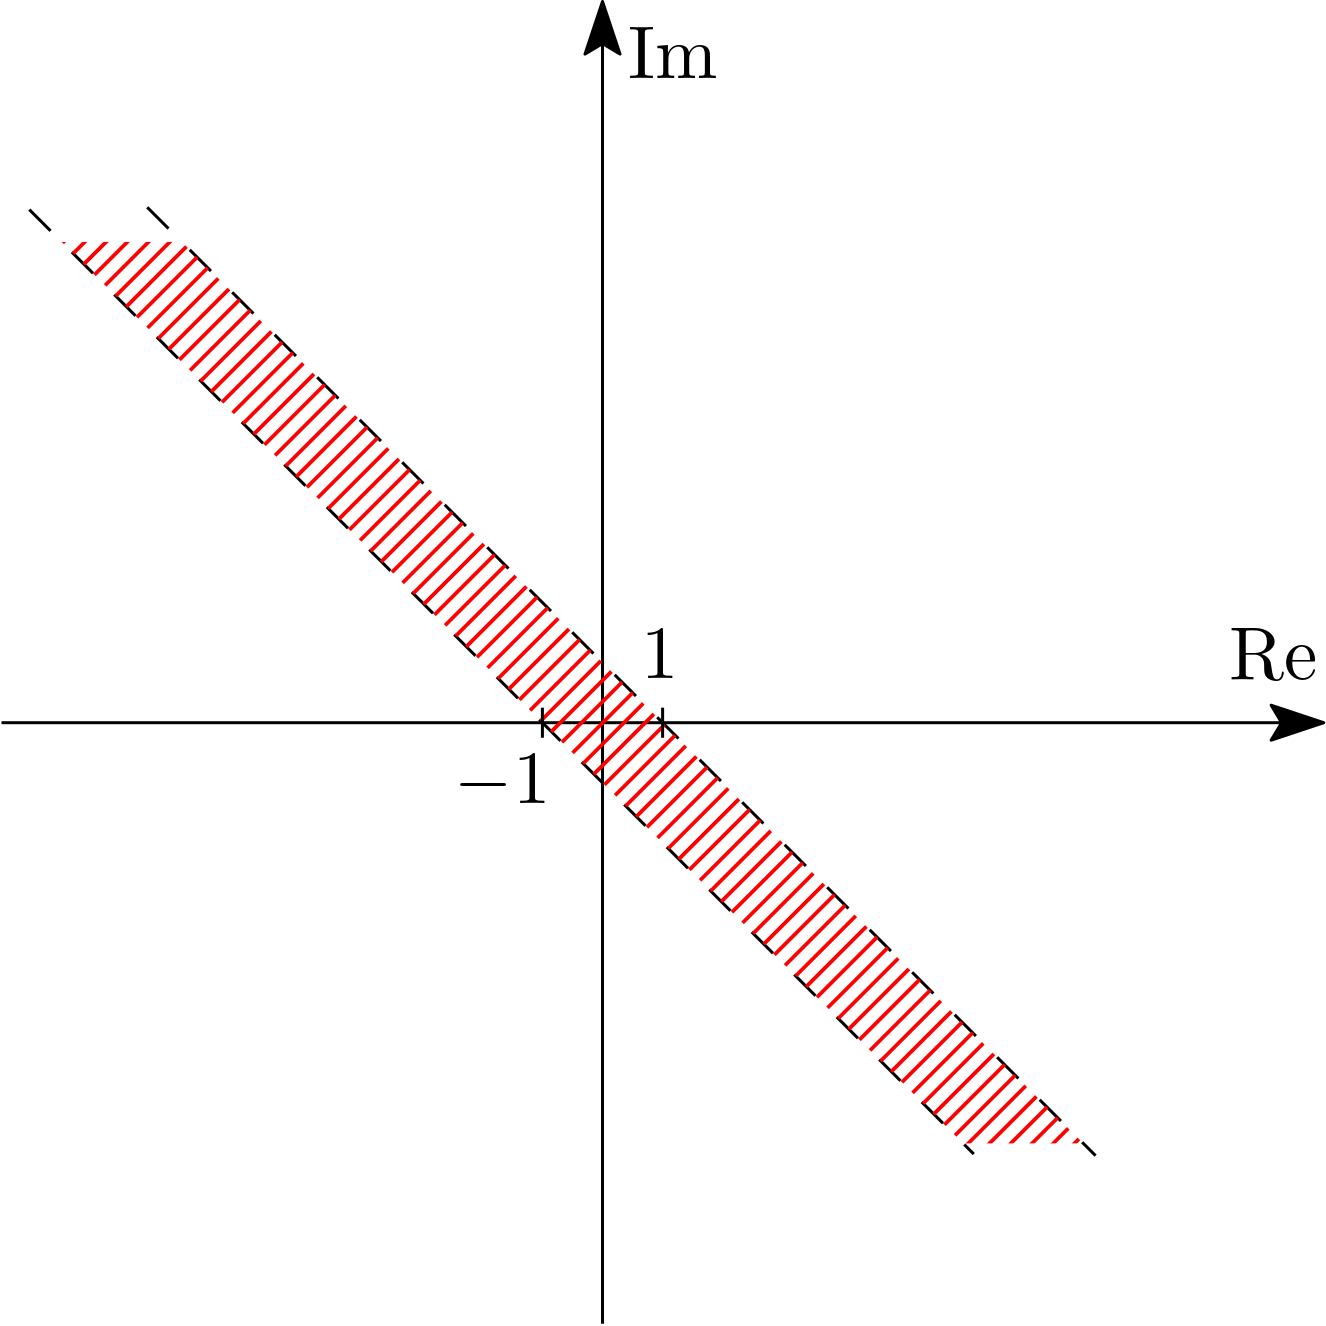
\includegraphics[width=0.3\textwidth]{AL1S2_1.png}
		\label{2_1}
		\caption{Область плоскости.}
	\end{figure}

	н) По определению, эллипс это ГМТ, таких, что сумма расстояний до двух заданных точек (называемых фокусами) равна константе. Фокусы в точках $-1$ и $1$, $a = \tfrac{3}{2}$, $e = \tfrac{c}{a} = \tfrac{1}{\tfrac{3}{2}} = \tfrac{2}{3}$, $b = \tfrac{3}{2}\sqrt{1- \tfrac{4}{9}} = \tfrac{\sqrt{5}}{2} \Rightarrow$ получим эллпис с канонической формой записи для $z = x + iy$ в следующем виде:
	$$
		\dfrac{4x^2}{9} + \dfrac{4y^2}{5} = 1
	$$
	\begin{figure}[H]
		\centering
		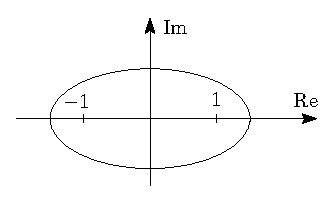
\includegraphics[width=0.25\textwidth]{AL1S2_2.eps}
		\label{2_2}
		\caption{Эллипс.}
	\end{figure}
\end{proof}

\begin{problem}(\textbf{К20.7} б))
 	$$
		\forall z,w \in \MC, \, 
		\begin{cases}
			z + w \in \MR\\
			z{\cdot}w \in \MR
		\end{cases} \Leftrightarrow
		\left[
			\begin{array}{l}
				z,w \in \MR \\
				z = \ovl{w}
			\end{array}
		\right.
	$$
\end{problem}
\begin{proof}\hfill\\
	$(\Leftarrow)$ $z,w \in \MR \Rightarrow z + w, z{\cdot}w \in \MR$ - очевидно. $z = \ovl{w} \Rightarrow z + w = 2\RE(w), \ovl{w}{\cdot}w = |w|^2 \in \MR$.
	$$
		z = a + bi,\, a,b \in \MR \Rightarrow \ovl{z} = a - bi \Rightarrow z + \ovl{z} = 2a, \, z{\cdot}\ovl{z} = a^2 + b^2 = |z|^2
	$$
	
	$(\Rightarrow)$ Пара чисел однозначно восстанавливается по их сумме и произведения, с точностью до перестановки. Тогда:
	$$
		z, w = \dfrac{z + 2 \pm(z- w)}{2} = \dfrac{z + w \pm \sqrt{D}}{2}
	$$
	$$
		(x - z)(x - w) = x^2 - (z + w)x + zw \Rightarrow D = (z + w)^2 - 4zw = (z - w)^2 
	$$
	$$
		z + w, z{\cdot}w \in \MR \Rightarrow D = (z -w)^2 \in \MR
	$$
	Единственное, мы не знаем какого знака получится $D$. Если меньше нуля, то возникают комплексные числа, если больше или равно нуля, то действительные. Рассмотрим эти случаи:
	\begin{enumerate}[label=\arabic*)]
		\item $D \geq 0 \Rightarrow z,w \in \MR$;
		\item $D < 0 \Rightarrow \sqrt{D} = \pm i\sqrt{|D|} \in \MC, \, \sqrt{|D|} \in \MR \Rightarrow z, w = \dfrac{z + 2 \pm(z- w)}{2} = \dfrac{z + w}{2} \pm i\dfrac{\sqrt{|D|}}{2} \Rightarrow z = \ovl{w}$;
	\end{enumerate}
\end{proof}

\subsection*{Поле комплексных чисел}
В прошлый раз мы ввели: $\MC = \MR + i \MR = \{a + bi \mid a,b\in \MR\}$, ввели операции: $+, -, \cdot, \div$ (не на ноль). Можно выполнить проверки, что сложение/умножение коммутативно, ассоциативно и умножение дистрибутивно, относительно сложения. Это означает, что $\MC$ - поле.
\begin{rem}
	Неформально говоря, поле - это множество на котором можно выполнять $4$ арифметические операации: $+, -, \cdot, \div$. Делить на ноль нельзя, всё остальное - можно. В поле обязательно есть два элемента: $0$ и $1$.
\end{rem}
\textbf{Примеры полей}: $\MQ \subset \MR \subset \MC$ - поля, $\MZ$ - не поле.  $\MC$ - самое большое числовое поле.
	
\subsection*{Извлечение корней из комплексных чисел}
Рассмотрим уравнение: $z^2 = w$ относительно $z$ при фиксированном $w$. В $\MR$ его можно решить только в случае, когда $w \geq 0$ и тогда возможно два случая:
\begin{enumerate}[label=\arabic*)]
	\item Тривиальный, когда $w = 0$; 
	\item Два решения, если $w > 0$, тогда  $z = \pm \sqrt{w}$, где $\sqrt{w} \geq 0$;
\end{enumerate}
В $\MC$ ситуация немного другая: 
$$
	z^2 = i = \sqrt{-1 } \Leftrightarrow z = \pm \dfrac{1 + i}{\sqrt{2}} \Rightarrow \sqrt{i} = \left\{\pm \dfrac{1 + i}{\sqrt{2}}\right\}
$$
Вообще говоря, корнем из $w$ мы называем множество: $\sqrt{w} = \{z \mid z^2 = w\}$.
\newpage
\begin{exrc}
	Из любого $w \neq 0 \in \MC$ можно извлечь корень, причем двумя способами.
\end{exrc}
\begin{proof}
	$$
		z = x + iy = ?, \, w = a+ ib, \, (x + iy)^2 = x^2 - y^2 + 2xyi = a + ib \Leftrightarrow 
		\begin{cases}
			x^2 - y^2 = a\\
			2xy = b
		\end{cases}
	$$
	Предположим, что $b \neq 0 \Rightarrow x,y \neq 0$, тогда:
	$$
		x = \dfrac{b}{2y} \Rightarrow \dfrac{b^2}{4y^2} - y^2 = a \Rightarrow y^4 + ay^2 - \dfrac{b^2}{4} = 0 \Rightarrow D = a^2 + b^2 = |w|^2 \Rightarrow y^2 = \dfrac{-a \pm \sqrt{a^2 + b^2}}{2} \in \MR \Rightarrow
	$$
	$$
		\Rightarrow y^2 = \dfrac{-a + \sqrt{a^2 + b^2}}{2} \Rightarrow y = \pm \sqrt{\dfrac{-a + \sqrt{a^2 + b^2}}{2}}, \, x = \pm \dfrac{b}{\sqrt{-2a + 2\sqrt{a^2 + b^2}}}
	$$
	Если $b = 0 \Rightarrow$ или $x = 0$ или $y = 0$, тогда:
	$$
		a < 0 \Rightarrow x^2 - y^2 < 0 \Rightarrow x = 0, -y^2 < 0 \Rightarrow y = \pm \sqrt{-a}
	$$
	$$
		a > 0 \Rightarrow x^2 - y^2 > 0 \Rightarrow  y = 0, x^2 > 0 \Rightarrow x = \pm \sqrt{a}
	$$
\end{proof}
Корень $n$-ой степени из $w$ определяется аналогично: $\sqrt[n]{w} = \{z \mid z^n = w\}$. Хотелось бы понять, можем ли мы алгебраически извлечь корень? Для простоты попробуем взять $n = 3$:
$$
	(x + iy)^3 = a + bi \Rightarrow (x + iy)^3 =  x^3 - 3xy^2 + i(3x^2y -y^3) \Rightarrow
	\begin{cases}
		a = x^3 - 3xy^2\\
		b = 3x^2y -y^3
	\end{cases}
$$
Как такое решать пока не очень ясно, если $a = 0$ или $b = 0$, то задача легко решается, поскольку расщепляется соответствующее уравнение. В общем виде - не очень ясно. Попробуем разобрать немного другую задачу.

\subsection*{Корни из единицы (примеры)}
Рассмотрим другую задачу, извлечем корень из $1$. Какие корни мы можем вычислить чисто алгебраически?
\begin{enumerate}[label=\arabic*)]
	\item $n = 2$:
	$$
		x^2 - 1 = (x - 1)(x + 1) \Rightarrow x = \sqrt{1} = \{\pm 1\}
	$$
	где $\sqrt{1} = \{\pm 1\}$ - комплексный корень в смысле определения: 
	$$
		\sqrt[n]{w} = \{z \mid z^n = w\}
	$$
	\item $n=3$:
	$$
		x^3  - 1 = (x - 1)(x^2 + x + 1) \Rightarrow x^2 + x + 1 = x^2 + x + \tfrac{1}{4} + \tfrac{3}{4} = \left(x + \tfrac{1}{2}\right)^2 - \left(\tfrac{i\sqrt{3}}{2}\right)^2 \Rightarrow
	$$
	$$
		\Rightarrow x^3  - 1 = (x - 1)\left(x + \tfrac{1}{2} - \tfrac{i\sqrt{3}}{2}\right)\left(x + \tfrac{1}{2} + \tfrac{i\sqrt{3}}{2}\right)\Rightarrow \sqrt[3]{1} = \left\{1, \dfrac{-1 \pm i\sqrt{3}}{2}\right\}
	$$
	геометрически, мы получаем правильный треугольник, где корни - его вершины;
	\begin{figure}[H]
		\centering
		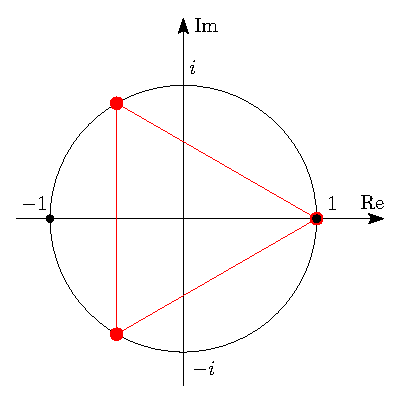
\includegraphics[width=0.3\textwidth]{AL1S2_3.eps}
		\label{2_3}
		\caption{Корень из единицы (черные точки) и кубический корень из единицы (красные точки).}
	\end{figure}
	\item $n = 4$:
	$$
		x^4 - 1 = (x^2 - 1)(x^2 + 1) = (x - 1)(x+1)(x -i)(x + i) \Rightarrow \sqrt[4]{1} = \{\pm 1, \pm i\}
	$$
	геометрически, мы получаем квадрат, где корни - его вершины;
	\item $n = 6$:
	$$
		x^6 - 1 = (x^3 - 1)(x^3 + 1) = -(x^3 - 1)((-x)^3 - 1) \Rightarrow \sqrt[6]{1} = \sqrt[3]{1} \cup \sqrt[3]{-1} = \sqrt[3]{1} \cup -\sqrt[3]{1} \Rightarrow
	$$
	$$
		\Rightarrow \sqrt[3]{1} = \left\{\pm 1, \dfrac{-1 \pm i\sqrt{3}}{2}, \dfrac{-1 \mp i\sqrt{3}}{2}\right\}
	$$
	геометрически, мы получаем правильный $6$-ти угольник, где корни - его вершины и корни $-\sqrt[3]{1}$ - противоположные корни $\sqrt[3]{1}$;
	\begin{figure}[H]
		\centering
		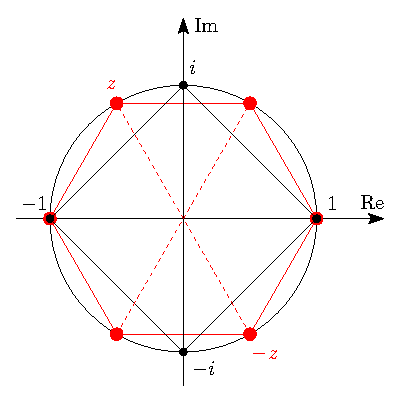
\includegraphics[width=0.3\textwidth]{AL1S2_4.eps}
		\label{2_4}
		\caption{$\sqrt[4]{1}$ (черные точки) и $\sqrt[6]{1}$ (красные точки).}
	\end{figure}
	\item $n = 8$:
	$$
		\sqrt[8]{1} = \sqrt[4]{1} \cup \sqrt[4]{-1} = \sqrt[4]{1} \cup \sqrt{\sqrt{-1}} =  \sqrt[4]{1} \cup \sqrt{i} \cup \sqrt{-i} \Rightarrow \sqrt[8]{1} = \left\{\pm 1, \pm i, \pm \dfrac{1 + i}{\sqrt{2}}, \pm \dfrac{1 - i}{\sqrt{2}}
		\right\}
	$$
	где $\sqrt{-1} = \{\pm i\} = \{z \mid z^2 = - 1\} \Rightarrow \sqrt{\sqrt{-1}} = \sqrt{i} \cup \sqrt{-i} = \{z \mid z^2 = \sqrt{-1}\}$. Геометрически, мы получаем правильный $8$-ми угольник, где корни - его вершины;
	\begin{figure}[H]
		\centering
		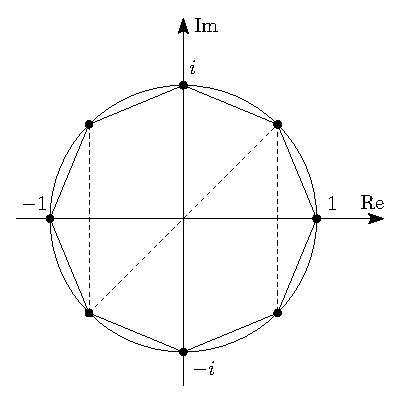
\includegraphics[width=0.3\textwidth]{AL1S2_5.eps}
		\label{2_5}
		\caption{$\sqrt[8]{1}$.}
	\end{figure}
\end{enumerate}
\begin{rem}
	Для уравнения $x^3 = 1$ в $\MR$ мы говорили, что $y = x^3$ - строго возрастает $\Rightarrow$ кроме единицы другого корня у этого уравнения нет. Тогда как в $\MC$ такие рассуждения уже не работают из-за того, что нельзя ввести порядок, согласованный с операциями.
\end{rem}
\begin{rem}
	Геометрически, противоположное комплексное число - будет лежать центрально симметрично, относительно $0$.
\end{rem}
Как быть с правильным $5$-угольником? Можно попробовать, но это алгебраический частный случай. И дальше хотелось бы понять, как можно извлекать корни $\Rightarrow$ нам нужно новое видение комплексных чисел, геометрическое.

Когда мы рассматриваем произведение положительных чисел это можно интерпритировать, как площадь прямоугольника. Какой геометрический смысл у $(-1){\cdot}(-1) = 1$ и $i^2 = -1$? 
\begin{enumerate}[label=(\arabic*)]
	\item $(-1){\cdot}(-1) = 1 \Rightarrow$ Если мы представим числа, как гомотетию, то есть растяжение, то тогда: $5$ - растяжение в пять раз, $\tfrac{1}{2}$ - сжатие в два раза. В этом смысле $-1$ - это центральная симметрия. Применение двух раз симметрии возвращает нас в исходное состояние;
	\begin{figure}[H]
		\centering
		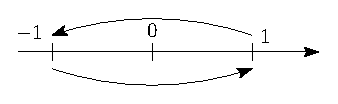
\includegraphics[width=0.25\textwidth]{AL1S2_6.eps}
		\label{2_6}
		\caption{Геометрический смысл $(-1)(-1) = 1$.}
	\end{figure}
	\item $i^2 = -1 \Rightarrow$ Нам необходима операция, которая при повторении дает симметрию, то есть поврот на $180^\circ$. Такой операцией является поворот на $90^{\circ} \Rightarrow$ умножение на $i$ это поворт на $90^{\circ}$; 
	\begin{figure}[H]
		\centering
		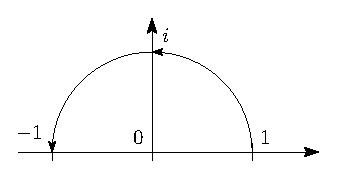
\includegraphics[width=0.25\textwidth]{AL1S2_7.eps}
		\label{2_7}
		\caption{Геометрический смысл $i^2 = -1$.}
	\end{figure}
\end{enumerate}

\subsection*{Геометрия умножения на комплексное число}
\textbf{\uline{Частный случай}}: Рассмотрим частный случай - умножение на $i$: $z \mapsto iz$.
\begin{rem}
	Такой стрелочкой с вертикальной чертой показывают куда переходит аргумент при отображении. Пусть $X, Y$ - множества, тогда отображение из $X$ в $Y$ записывается так: 
	$$
		f \colon X \to Y
	$$ 
	Когда же мы рассматриваем аргументы, то запись имеет вид:
	$$
		f \colon x \mapsto f(x) = y
	$$
\end{rem}
Мы хотим показать, что $z \mapsto iz$ - поворот на $90^{\circ}$ против часовой стрелки. Пусть $z = a + ib$, тогда: $$
	\forall z \in \MC, \, z = a + ib \Rightarrow iz = ia + bi^2 = ia - b = -b + ia
$$
\begin{figure}[H]
	\centering
	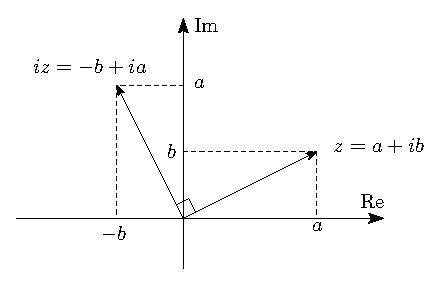
\includegraphics[width=0.4\textwidth]{AL1S2_8.eps}
	\label{2_8}
	\caption{Геометрический смысл умножения на $i$.}
\end{figure}

\textbf{\uline{Общий случай}}: 
\begin{enumerate}[label=\arabic*)]
	\item \uwave{Алгебраическая форма записи} комплексного числа соответствует декартовой системе координат: действительная часть - абсцисса, мнимая - ордината:
	$$
		z = x + yi
	$$
	\item \uwave{Тригонометрическая форма записи} комплексного числа соответствует полярной системе координат: каждая точка (кроме начала координат) определяется расстоянием до нуля и углом, который образует этот вектор с положительной полуосью абсцисс:
	$$
		z = r(\cos\varphi + i\sin\varphi), \, z \neq 0, \, r = |z| > 0, \, \varphi = \arg(z)
	$$
	где $\arg(z)$ - аргумент комплексного числа, определен с точностью до $2\pi k,\, k \in \MZ$;
\end{enumerate} 
\begin{rem}
	Заметим, что на окружности радиуса единица: $r = 1$, значение комплексных чисел будет равно: $z = \cos\varphi + i\sin\varphi$. Это есть ничто иное, как определение косинуса и синуса: косинус - абсцисса, синус - ордината. Любое произвольное комплексное число получается из числа на единичной окружности каким-то растяжением или сжатием.
\end{rem}
\begin{figure}[H]
	\centering
	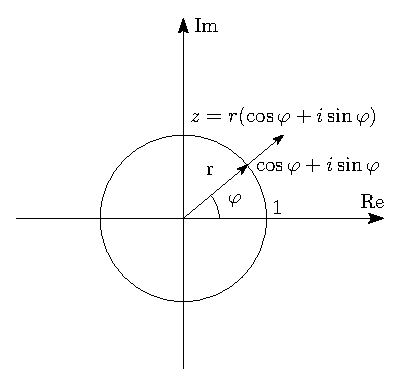
\includegraphics[width=0.4\textwidth]{AL1S2_9.eps}
	\label{2_9}
	\caption{Тригонометрическая форма записи комплексного числа.}
\end{figure}
\begin{problem}(\textbf{К21.1})
	Найти тригонометрическую форму:
	
	а) $5 \Rightarrow 5 = 5{\cdot}(1 + i{\cdot}0) = 5{\cdot}(\cos0 + i\sin0)$;
	
	б) $i \Rightarrow i = 1{\cdot}(0 + i{\cdot}1) = 1{\cdot}\left(\cos\tfrac{\pi}{2} + i\sin{\tfrac{\pi}{2}}\right)$;
	
	д) $1 + i \Rightarrow 1 + i = \sqrt{2}{\cdot}\left(\cos\tfrac{\pi}{4} + i \sin\tfrac{\pi}{4}\right)$;
	
	з) $-1 + i\sqrt{3} \Rightarrow -1 + i\sqrt{3} = 2{\cdot}\left(\cos\tfrac{2\pi}{3} + i \sin\tfrac{2\pi}{3}\right)$;
	
	с) $1 - (2 + \sqrt{3})i \Rightarrow |1 - (2 + \sqrt{3})i| =  2\sqrt{2 + \sqrt{3}}$, угол же найдется через арктангенс: $\varphi = -\arctg(2 + \sqrt{3})$. Чтобы найти его значение в явном виде, решим задачу по поиску угла на следующей картинке:
	\begin{figure}[H]
		\centering
		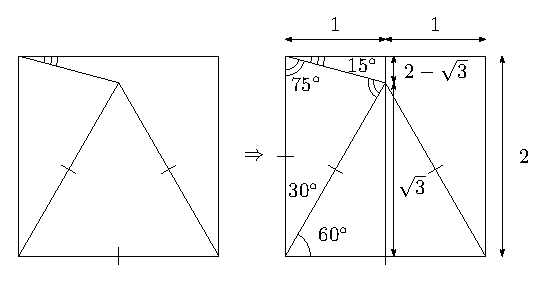
\includegraphics[width=0.5\textwidth]{AL1S2_10.eps}
		\label{2_10}
		\caption{Нахождение угла $\varphi = -\arctg(2 + \sqrt{3})$.}
	\end{figure}
	По картинке, мы можем увидеть, что $\tg15^{\circ} = 2 - \sqrt{3}, \, \ctg15^{\circ} = \tg75^{\circ} = 2 + \sqrt{3} \Rightarrow$ мы можем задать аргумент в явном виде:
	$$
		\varphi = -\arctg(2 + \sqrt{3}) = -75^{\circ} = -\dfrac{5\pi}{12}
	$$ 
	
	т) $\cos(\alpha) - i\sin(\alpha) \Rightarrow \cos(\alpha) - i\sin(\alpha) = \cos(-\alpha) + i\sin(-\alpha)$;
\end{problem}
\newpage
\begin{theorem}
	Отображение $f\colon z \mapsto r(\cos\varphi + i\sin\varphi){\cdot}z, \, r > 0, \, \varphi \in \MR$ является композицией (в любом порядке) двух отображений плоскости:
	\begin{enumerate}[label=\arabic*)]
		\item \uline{Гомотетия} с коэффициентом $r$ с центром в $0$;
		\item \uline{Поворт} на угол $\varphi$ с центром в $0$;
 	\end{enumerate}
\end{theorem}
\textbf{Пример}: $z \mapsto (1 + i)z$ - гомотетия с коэффициентоам $\sqrt{2}$ плюс поворот на $\tfrac{\pi}{4}$.
\begin{proof}
	Пусть $z \neq 0$, запишем его в тригонометрическом виде:
	$$
		z = R(\cos\alpha + i\sin\alpha)\Rightarrow f(z) = R{\cdot}r{\cdot}(\cos\alpha + i\sin\alpha){\cdot}(\cos\varphi + i\sin\varphi) = 	
	$$
	$$
		=Rr(\cos\alpha \cos\varphi +i\cos\alpha\sin\varphi + i\sin\alpha\cos\varphi - \sin\alpha\sin\varphi) = Rr(\cos(\alpha + \varphi) + i\sin(\alpha + \varphi)) \Rightarrow
	$$
	$$
		\Rightarrow |R| \mapsto |R|{\cdot}|r|, \, \arg(z) = \alpha \mapsto \arg(f(z)) = \alpha + \varphi
	$$
	Таким образом, получили растяжение и поворот на $\varphi$.
\end{proof}

\begin{corollary}(\textbf{формула Муавра $\RN{1}$, $1707$})
	$$
		(\cos\alpha + i\sin\alpha)^n = \cos(n\alpha) + i\sin(n\alpha), \, n\in\MZ, \, \alpha \in \MR
	$$
\end{corollary}
\begin{proof}
	Повернуть угол на $\alpha$ $n$ раз это тоже самое, что и сразу повернуть угол на $n\alpha$. Отдельный случай для $n = -1$:
	$$
		\dfrac{1}{\cos\alpha + i\sin\alpha} = \dfrac{\cos\alpha - i\sin\alpha}{\cos^2\alpha - i^2\sin^2\alpha} = \cos\alpha - i\sin\alpha = \cos(-\alpha) + i\sin(-\alpha)
	$$
	Дальше по индукции верно для любого $n$.
\end{proof}

\begin{problem}(\textbf{К21.2})
	
	а) $(1 + i)^{1000} = ((1 +i)^2)^{500} = (2i)^{500} = 2^{500}$ - алгебраический способ, но такое решение будет не всегда.
	$$
		(1 + i)^{1000} = \left(\sqrt{2}\left(\cos\tfrac{\pi}{4} + i\sin{\pi}{4} \right)\right)^{1000} = 2^{500}(\cos(250\pi) + i\sin(250\pi)) = 2^{500}
	$$
	
	в) $(\sqrt{3} + i)^{30} = \left(2\left(\cos\tfrac{\pi}{6} + i\sin\tfrac{\pi}{6}\right)\right)^{30} =2^{30}\left(\cos(5\pi) + i\sin(5\pi) \right) = -2^{30}$;
	
	е) $\left(\dfrac{1 - i\sqrt{3}}{1 + i}\right)^{12} = z \Rightarrow |1 - i\sqrt{3}| = \sqrt{4} = 2, \, |1 +i| = \sqrt{2}$ найдем в отдельности модуль и аргумент $z$:
	$$
		|z| = \dfrac{|1 - i\sqrt{3}|}{|1 + i|} = \sqrt{2} \Rightarrow |z|^{12} = 2^6 = 64
	$$
	$$
		\dfrac{\cos\alpha + i\sin\alpha}{\cos\beta + i\sin\beta} = (\cos\alpha + i \sin\alpha)(\cos(-\beta) + i\sin(-\beta)) = \cos(\alpha - \beta) + i\sin(\alpha - \beta) \Rightarrow
	$$
	$$
		\Rightarrow \arg(1 - i\sqrt{3}) = - \dfrac{\pi}{3}, \, \arg(1 + i) = \dfrac{\pi}{4}, \, \arg\left(\dfrac{1 - i\sqrt{3}}{1 + i}\right) = -\dfrac{\pi}{3} - \dfrac{\pi}{4} = -\dfrac{7\pi}{12} \Rightarrow 
	$$
	$$	
		\Rightarrow \left(\dfrac{1 - i\sqrt{3}}{1 + i}\right)^{12}  =64(\cos(-7\pi) + i\sin(-7\pi)) = 64(\cos\pi + i\sin\pi)= -64
	$$
	где $\modn{-7\pi}{\pi}{2\pi}$.
\end{problem}

\newpage
\subsection*{Извлечение корней из комплексных чисел}
Как мы уже говорили: $\sqrt[n]{w} = \{z \mid z^n = w\}$. Как будем находить корни? Сначала, перепишем всё в тригонометрических терминах.
$$
	w = R(\cos\alpha + i\sin\alpha) \neq 0, \, z = r(\cos\varphi + i\sin\varphi) \neq 0
$$
Нам дано $w$ и $n \in \MZ$, необходимо найти $z$:
$$
	z^n = w \Leftrightarrow r^n(\cos(n\varphi) + i\sin(n\varphi)) = R(\cos\alpha + i \sin\alpha) \Leftrightarrow 
$$	
$$
	\Leftrightarrow
	\begin{cases}
		r^n = R\\
		n\varphi = \alpha + 2\pi k, \, k \in \MZ
	\end{cases}
	\Leftrightarrow 
	\begin{cases}
		r = \sqrt[n]{R} \in \MR\\
		\varphi = \dfrac{\alpha + 2\pi k}{n}, \, k \in \MZ
	\end{cases}
$$
\begin{theorem}(\textbf{формула Муавра $\RN{2}$, $1707$})
	$\forall R > 0, \, \alpha \in \MR$ справедлива формула:
	$$
		\sqrt[n]{R(\cos\alpha + i \sin\alpha)} = \left\{\sqrt[n]{R}\left( \cos\tfrac{\alpha + 2\pi k}{n} + i\sin\tfrac{\alpha + 2\pi k}{n}\right) \mid k = 0,1, \dotsc, n-1\right\}
	$$
	Это $n$ точек, лежащих на окружности радиуса $\sqrt[n]{R}$ в вершинах правильного $n$-угольника.
\end{theorem}
\begin{rem}
	Точки указанные в формуле будут повторяться с периодичностью в $2\pi$.
\end{rem}

\begin{problem}(\textbf{К22.6} б))
	Найти корни: $\sqrt[10]{512(1 - i\sqrt{3})}$:
	$$
		\sqrt[10]{512(1 - i\sqrt{3})} = \sqrt[10]{2^{10}\left(\cos\left(-\tfrac{\pi}{3}\right) + i\sin\left(-\tfrac{\pi}{3}\right)\right)} = \left\{2\left( \cos\left(-\tfrac{\pi}{30} + \tfrac{\pi k}{5}\right) + i\sin\left(-\tfrac{\pi}{30} + \tfrac{\pi k}{5}\right)\right)  \mid k = 0, \dotsc,9\right\}
	$$
\end{problem}

\textbf{ДЗ}: $20.8$б, $20.10$б, $21.1$влух, $21.2$вж, $21.9$вг, $21.10$, $22.1$, $22.2$, $22.5$, $22.6$, $22.7$aвзио
\end{document}